	\subsection{Resultados da Simulação}
	\label{subsec:resultadoSimulacao}

	Diversas simulações foram realizadas no simulador GRUBiX, como descrito na Seção \ref{subsec:simulacao}. As simulação foram realizadas para avaliar o comportamento do agente em redes com diferentes níveis de densidade de nós e distância de comunicação dos nós. Outra situação simulada foi redes somente com veículos sem uma infraestrutura de apoio e outra híbrida.

	Após realizar as simulações os dados foram organizados e analisados em três fases:

	\begin{enumerate}
		\item Resultados obtidos na rede sem infraestrutura
		\item Resultados obtidos na rede híbrida
		\item Comparação dos resultados obtidos nas duas situações
	\end{enumerate} 

	\subsubsection{Rede sem infraestrutura}
	\label{subsubsection:redeSemInfraestruturaResultadoDiscucao}

	Os resultados obtidos da rede sem infraestrutura mostram que o raio de alcance e a quantidade dos nós afetam o desempenho do agente. A Figura \ref{fig:graficosSemTorres} demonstra a evolução do tempo que o agente permaneceu na região alvo com o aumento do raio e a quantidade de nós. 

	\begin{figure}[htbp]
		\centering
		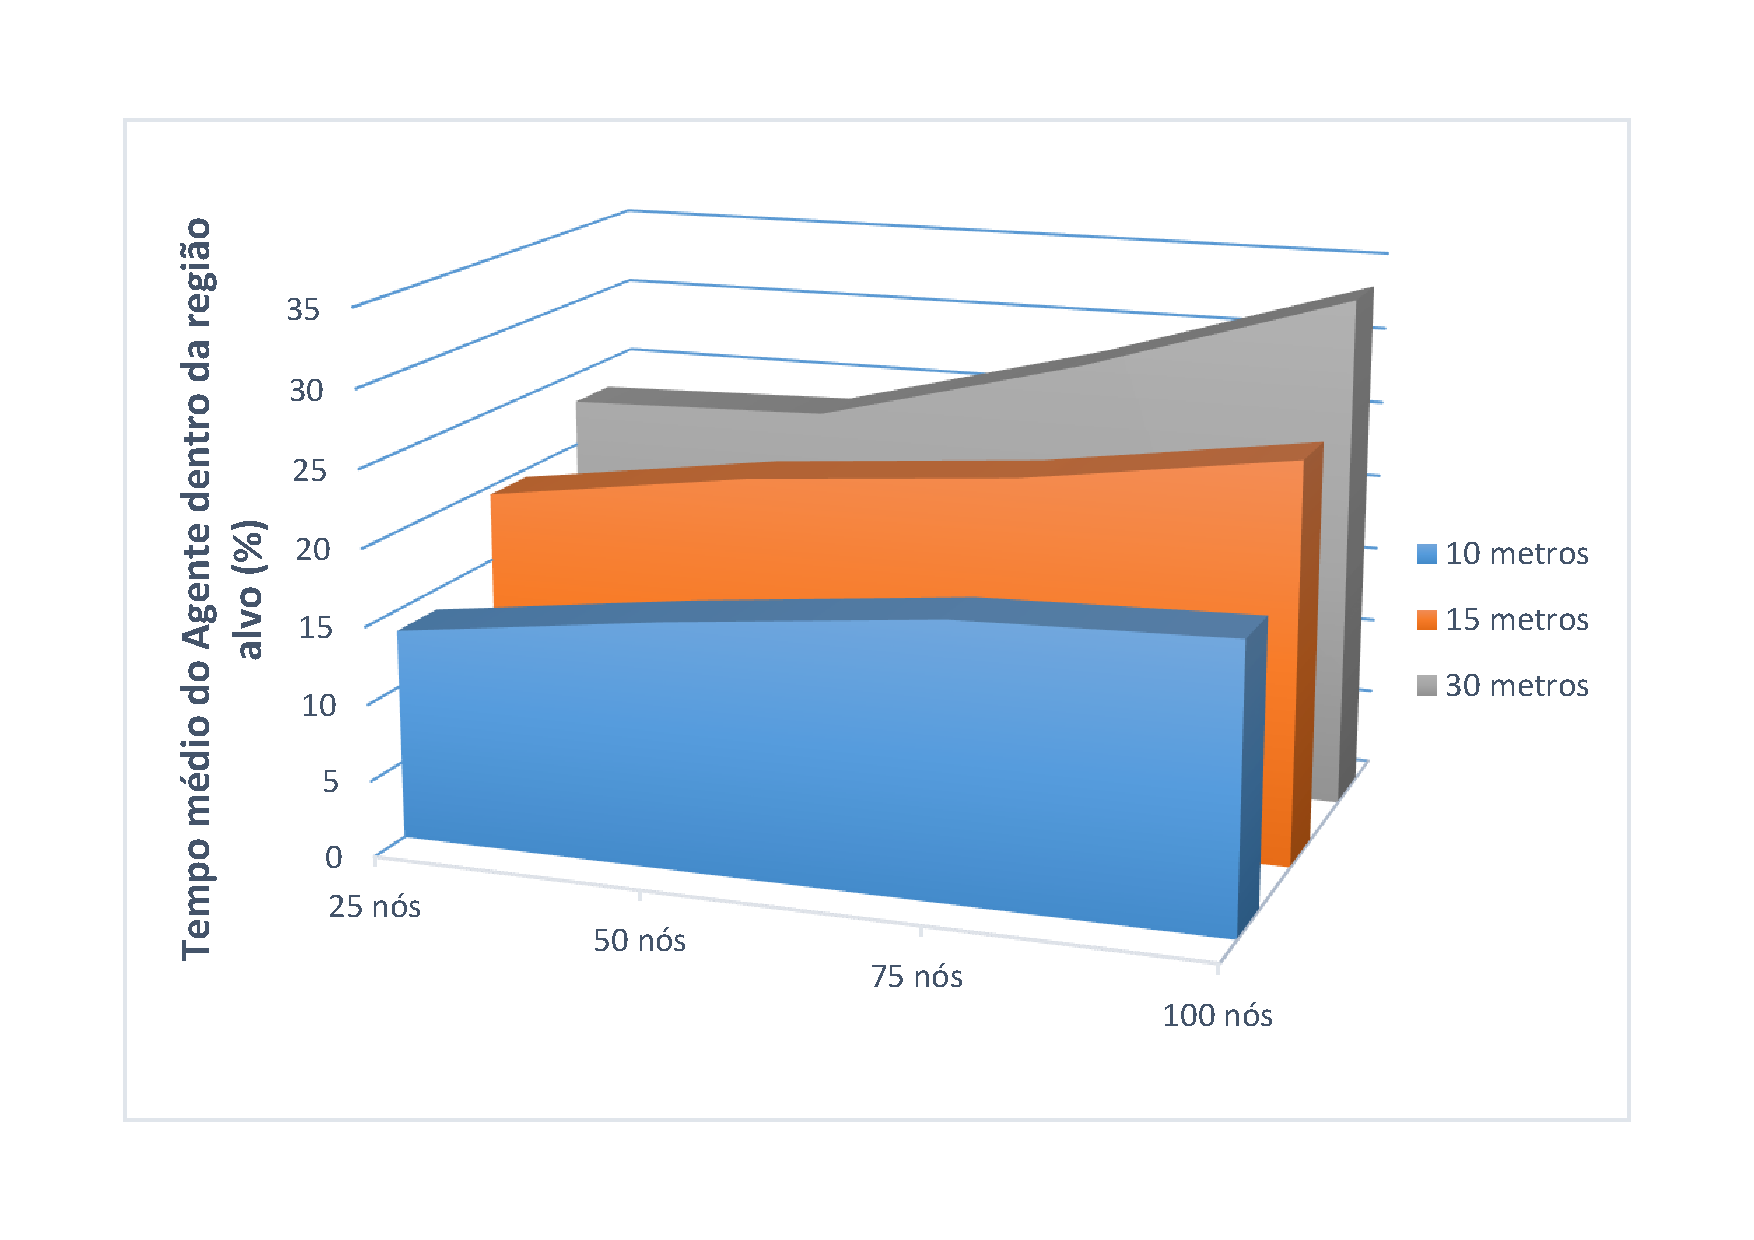
\includegraphics[scale=0.34]{resultados/graficos/graficoSemTorres.pdf}
		\caption{Resultados obtidos no cenários sem infraestrutura.}
		\label{fig:graficosSemTorres}
	\end{figure}

	Na Tabela \ref{tab:estatiscaResultadosObtidosSemInfraestrutura} é possível visualizar a média aritmética, o desvio padrão e a variância dos resultados obtidos. 

	\begin{table}[!htb]
	    \caption{Estátistica dos resultados obtidos}
	    \label{tab:estatiscaResultadosObtidosSemInfraestrutura}
	    \centering
	    \tiny
	    \begin{minipage}{.5\linewidth}
	      
	      \centering
	        \begin{tabular}{|c|c|c|c|}

			\hline
			\multicolumn{4}{|c|}{25 nós} \\ \hline
			Alcance   & média aritmetica &	Desvio Padrão &	Variância  \\ \hline
			10 metros &	13,6767 & 2,2579 &	5,2766  \\ \hline
			15 metros &	19,4554 & 1,7157 &	3,3192  \\ \hline
			30 metros &	23,0320 & 0,8125 &	1,1901 \\ \hline

			\multicolumn{4}{|c|}{} \\ \hline

			\multicolumn{4}{|c|}{50 nós} \\ \hline
			Alcance   & média aritmetica &	Desvio Padrão &	Variância  \\ \hline
			10 metros &	15,9696	& 1,4147 & 2,2524  \\ \hline
			15 metros &	21,9589	& 1,4315 & 2,5295  \\ \hline
			30 metros &	23,4864	& 1,1216 & 1,8084 \\ \hline

		\end{tabular}
	    \end{minipage}%
	    \begin{minipage}{.5\linewidth}
	      \centering
	        \begin{tabular}{|c|c|c|c|}
	        \hline
			\multicolumn{4}{|c|}{75 nós} \\ \hline
			Alcance   & média aritmetica &	Desvio Padrão &	Variância  \\ \hline
			10 metros &	17,8484 & 2,6340 & 7,2524  \\ \hline
			15 metros &	23,4404 & 2,3308 & 5,9770  \\ \hline
			30 metros &	28,0170 & 1,4151 & 2,7856 \\ \hline

			\multicolumn{4}{|c|}{} \\ \hline


			\multicolumn{4}{|c|}{100 nós} \\ \hline
			Alcance   & média aritmetica &	Desvio Padrão &	Variância  \\ \hline
			10 metros &	18,4040	& 2,8614 & 8,5221  \\ \hline
			15 metros &	26,0110	& 1,4059 & 2,6514  \\ \hline
			30 metros &	33,4824	& 1,1032 & 2,3361 \\ \hline

		\end{tabular}

	    \end{minipage} 
	\end{table}

A cada vinte e cinco nós que são adicionados a rede a eficiência do agente aumenta em 11,53\%. Quando o aumento ocorre no raio do alcance do nó a melhora do desempenho é de 28,38\%. O aumento entre o alcance de 10 metros e 15 metros foi maior (37,88\%) que o aumento de 15 metros para 30 metros (18,87\%). 

Isso ocorre por que com o aumento do raio somente uma pequena parte do aumento fica sobre a rua onde estão os veículos. A Figura \ref{fig:problemaDisperdicio} demonstra o problema, a região vermelha é a representação da região onde o sinal é disperdiçado. Quando maior o raio de alcance do nó maior o disperdicio, essa é uma desvantagem em não usar rede híbrida. Por que dentro das quadras poderiam ter outros dispositivos que auxiliariam o agente, assim o agente poderia encontrar rotas através das quadras, aumentando a quantidade de rotas disponíveis para ele usar.

\begin{figure}[htbp]
		\centering
		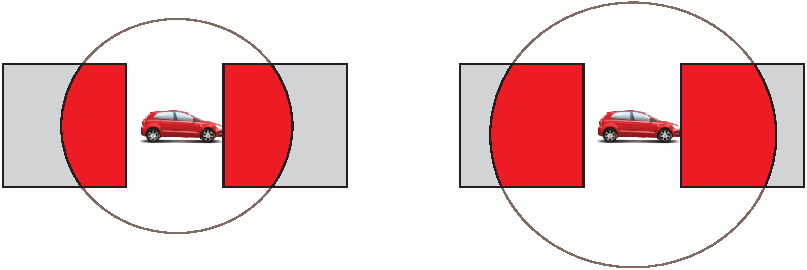
\includegraphics[scale=0.5]{resultados/figuras/problemaDisperdicio.pdf}
		\caption{Exemplificação do disperdicio.}
		\label{fig:problemaDisperdicio}
	\end{figure}

Como o veículo não é necessário realizar uma economia de energia, o alcance da comunicação dos nós podem ser alta, isso melhora o desempenho do agente. 

Quanto maior é a quantidade de veículos o agente alcançar ao buscar novos nós hospedeiros, maior as chances dele cumprir a missão. A melhora em comparação entre a situação onde o agente tem a disposição o menor alcance e a menor densidade de veículospara a situação mais farta de recursos é de 144,81\%.   





\subsubsection{Rede com infraestrutura}

	Os dados obtidos em uma rede veícular com infraestrutura demonstrou que a densidade e raio de alcance tem os mesmos impactos discutidos na Seção 
	\ref{subsubsection:redeSemInfraestruturaResultadoDiscucao}.

	Na Figura \ref{fig:graficosComTorres} demonstra a melhoria de desempenho do agente ao aumentar a densidade dos nós e o raio de alcance. A melhoria de desempenho do agente na configuração com a menor quantidade de recursos para a rede com a configuração com maior quantidade de recursos foi de 114,43\%.   
 

	\begin{figure}[htbp]
		\centering
		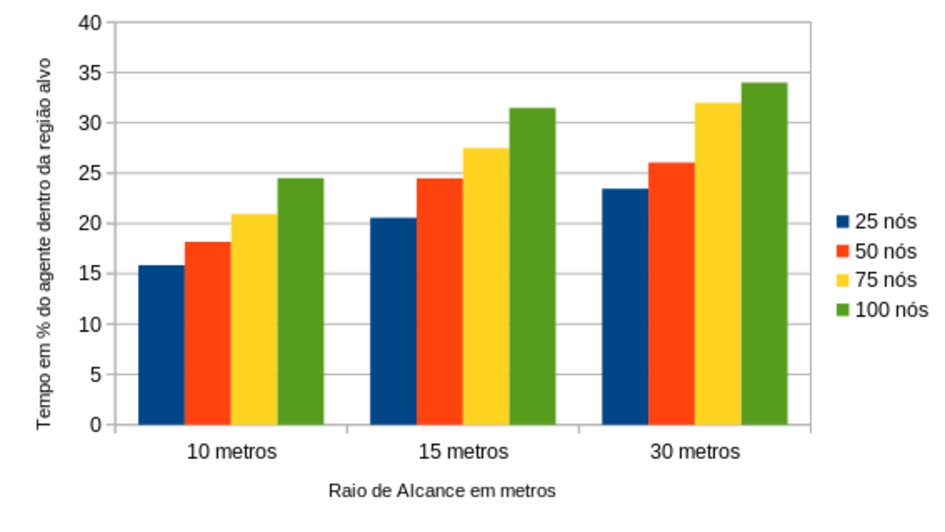
\includegraphics[scale=0.34]{resultados/graficos/graficoComTorres.pdf}
		\caption{Resultados obtidos no cenários com infraestrutura.}
		\label{fig:graficosComTorres}
	\end{figure}

	Para cada vinte e cinco nós que entram na rede, o agente melhora o seu desempenho em 14,56\%. O aumento do raio do nó causa um impacto de 20,94\%. Com o aumento do raio e a densidade causa impacto diretamente na quantidade de veículos que o agente tem acesso.

	Na Tabela \ref{tab:estatiscaResultadosObtidosComInfraestrutura} é possível visualizar a média aritmética, o desvio padrão e a variância dos resultados obtidos.

	\begin{table}[!htb]
	    \caption{Estátistica dos resultados obtidos}
	    \label{tab:estatiscaResultadosObtidosComInfraestrutura}
	    \centering
	    \tiny
	    \begin{minipage}{.5\linewidth}
	      
	      \centering
	        \begin{tabular}{|c|c|c|c|}

			\hline
			\multicolumn{4}{|c|}{25 nós} \\ \hline
			Alcance   & média aritmetica &	Desvio Padrão &	Variância  \\ \hline
			10 metros &	15,8585 & 1,4024 & 2,2208  \\ \hline
			15 metros &	20,5735 & 1,6888 & 3,2724  \\ \hline
			30 metros &	23,4544 & 1,1172 & 1,7970 \\ \hline

			\multicolumn{4}{|c|}{} \\ \hline

			\multicolumn{4}{|c|}{50 nós} \\ \hline
			Alcance   & média aritmetica &	Desvio Padrão &	Variância  \\ \hline
			10 metros &	18,1818 & 1,4338 & 2,3783  \\ \hline
			15 metros &	24,4884 & 1,1216 & 1,8565  \\ \hline
			30 metros &	26,0580 & 1,4123 & 2,6716 \\ \hline

		\end{tabular}
	    \end{minipage}%
	    \begin{minipage}{.5\linewidth}
	      \centering
	        \begin{tabular}{|c|c|c|c|}
	        \hline
			\multicolumn{4}{|c|}{75 nós} \\ \hline
			Alcance   & média aritmetica &	Desvio Padrão &	Variância  \\ \hline
			10 metros &	20,9494 & 2,0501 & 4,6422  \\ \hline
			15 metros &	27,5075 & 1,6945 & 3,6252  \\ \hline
			30 metros &	31,9959 & 1,3899 & 2,9536 \\ \hline

			\multicolumn{4}{|c|}{} \\ \hline


			\multicolumn{4}{|c|}{100 nós} \\ \hline
			Alcance   & média aritmetica &	Desvio Padrão &	Variância  \\ \hline
			10 metros &	24,5151 & 1,1021 & 1,8119  \\ \hline
			15 metros &	31,4934 & 1,1350 & 2,2770  \\ \hline
			30 metros &	34,0060 & 1,4240 & 3,1813 \\ \hline

		\end{tabular}

	    \end{minipage} 
	\end{table}  